% Hauptteil

\section{Simulation des Batteriespeichersystems}

In diesem Kapitel werden die wichtigsten Simulationsschritte dargestellt und erläutert. Weiterhin erfolgt eine Betrachtung der Ergebnisse.

\subsection{Parametervariation und Simulationsziele}

Die Parametervariation soll dazu dienen, möglichst viele Fälle möglichst genau darstellen zu können. Folgende Parameter fließen modellendogen in die Durchläufe der Simulation ein:

\begin{itemize}
\itemsep-0.5em
	\item Der Hausverbrauch von \SIrange{3000}{10000}{\kwh}
	\item Die Kapazität der Batterie von \SIrange{8}{16}{\kwh}
	\item Die Größe der Photovoltaikanlage von \SIrange{5.5}{10}{\kwp}
	\item Die EEG-Vergütung für die Stromeinspeisung von \SIrange{9.87}{12.75}{\ctkwh}
	\item Der Grundpreis des Vergleichstromtarifs von \SIrange{5}{12}{\Eurkwh}
	\item Der Arbeitspreis des Vergleichstromtarifs von \SIrange{25}{32}{\ctkwh}
\end{itemize}

\noindent Weiterhin sind folgende Parameter modellexogen vorgegeben und nicht variiert:

\begin{itemize}
\itemsep-0.5em
	\item Die nominale AC-Leistungsaufnahme des Batteriewechselrichters \SI{3.3}{\kw}
	\item Die nominale AC-Leistungsabgabe des Batteriewechselrichters \SI{3.3}{\kw}
	\item Der mittlerer Umwandlungswirkungsgrad des Batteriewechselrichters im Ladebetrieb \SI{94.4}{\percent}
	\item Der mittlerer Umwandlungswirkungsgrad des Batteriewechselrichters im Entladebetrieb \SI{94.5}{\percent}
	\item Der mittlerer Umwandlungswirkungsgrad des Batteriespeichers \SI{93.8}{\percent}
	\item Die präqualifizierte Leistung des virtuellen Kraftwerks $\pm \SI{1}{\mega\watt}$
	\item Die theoretische maximale Leistung des virtuellen Kraftwerks $\pm \SI{1.98}{\mega\watt}$
	\item Der sonnenBonus in Höhe von \SI{0.25}{\ctkwh}
\end{itemize}

\noindent Das Ziel der Simulation ist es, in erster Linie einen Kostenvergleich der Vertragsvarianten für den Kunden zu ermöglichen. Die wichtigsten zu ermittelten Größen sind von daher die jährlichen Kosten. Außerdem soll ermittelt werden, wie stark die Batterie durch das virtuelle Kraftwerk mehr belastet wird. Hierfür werden die auftretenden Vollzyklen pro Jahr berechnet.

\subsection{Simulation des Einflusses des virtuellen Kraftwerks}

Dieses Kapitel soll die Simulation des Einflusses des virtuellen Kraftwerks auf das eigenverbrauchsoptimierte Verhalten der Batterie erläutern. Weiterhin soll eine Bewertung der Approximation vorgenommen werden.

\subsubsection{Erläuterung der Simulation}

Die Erbringung von Primärregelleistung hat immer Vorrang vor der Eigenverbrauchsoptimierung des Kunden. Somit muss ermittelt werden, in welchen Zeitschritten es zu einer Erbringung von Primärregelleistung kommt.\medskip\\
Als erste Approximation wird angenommen, dass das virtuelle Kraftwerk an \SI{80}{\percent} der Tage des Jahres an der Erbringung von Primärregelleistung teilnimmt. Hierdurch werden Wartung und nicht erfolgreiche Ausschreibungen abgedeckt. Um einen ausreichenden Ladestand zu garantieren, wird weiterhin zwischen zwei Zuständen unterschieden:

\begin{enumerate}
\itemsep-0.5em
	\item Die Ladestandsgrenzen sind aktiviert
	\item Die Erbringung von Primärregelleistung und die Ladestandsgrenzen sind aktiviert
\end{enumerate}

\noindent Der erste Fall tritt immer dann auf, wenn auf einen Tag ohne Erbringung von Primärregelleistung ein regelleistungsaktiver Tag folgt. In diesem Fall werden die Ladestandsgrenzen von \SIrange{20}{80}{\percent} bereits \SI{12}{\hour} vor der eigentlichen Erbringung aktiviert. Damit soll möglichst sichergestellt werden, dass zu Beginn der Regelleistungserbringung genügend Energie in den Speichern zur Verfügung steht. Weiterhin soll auf diese Weise auf eine Simulation des Nachlademanagements des virtuellen Kraftwerks verzichtet werden können.\medskip\\
Im nächsten Schritt, muss ermittelt werden ob die eigene Batterie in dem vorliegenden Zeitschritt an der Erbringung von Primärregelleistung teilnimmt. Hierfür wurde ein einfacher boolean Minuten-Vektor geschaffen, mit folgenden Bedeutungen:

\begin{conditions}
	0		&		Eigenverbrauchsoptimierung\\
	1		&		Erbringung von Primärregelleistung\\
\end{conditions}

\noindent Damit die Batterie an der Regelleistungserbringung teilnimmt, muss die Regelleistungserbringung des gesamten virtuellen Kraftwerks aktiv sein, die Frequenzabweichung der Netzfrequenz außerhalb des Totbandes liegen und die Batterie zu den verwendeten Batterien des Zeitschritts gehören.\\
Um die letzte Vorraussetzung zu approximieren, wurde vorerst die Wahrscheinlichkeit berechnet, dass die Batterie Primärregelleistung in dem Zeitschritt erbringen muss.

\begin{equation}
\label{eq:approx_FCR}
	p_{\text{FCR}}\left(t\right) = \left|P_{\text{FCR}_{\text{VPP}}}\left(t\right)\right| \cdot \frac{P_{\text{PQ}}}{P_{\text{max}}}
\end{equation}

\begin{conditions}
	t															&		Zeitschritt\\
	p_{\text{FCR}}\left(t\right)					&		Wahrscheinlichkeit der Regelleistungserbringung\\
	P_{\text{FCR}_{\text{VPP}}}\left(t\right)	&		Abgerufene Primärregelleistung des virtuellen Kraftwerks im Zeitschritt\\
	P_{\text{PQ}}										&		Präqualifizierte Leistung des virtuellen Kraftwerks\\   
	P_{\text{max}}									&		Theoretische maximale Leistung des virtuellen Kraftwerks \\   
\end{conditions}

\noindent Der hierbei entstehende Vektor wird anschließend mit einem Vektor verglichen, dessen Variablen zufällig in einem Bereich von \SIrange{0}{100}{\percent} generiert wurden. Liegt der Wert der Approximation oberhalb der Zufallsvariable, wird in diesem Zeitschritt Primärregelleistung erbracht.\\
Dies gilt jedoch nur, wenn zeitgleich auch das virtuelle Kraftwerk aktiv ist. Werden die beiden Vektoren miteinander abgeglichen, ergibt sich, dass die Regelleistungserbringung der Batterie ca. \SI{3}{\percent} der Gesamtzeit ausmacht.

\subsubsection{Bewertung der Approximation}

Um die Approximation bewerten zu können, muss ein Optimum definiert werden. In der Simulation wird von einem homogenen virtuellen Kraftwerk ausgegangen. Das heißt, dass die Last genau gleichmäßig zwischen den Batterien aufgeteilt wird. Die theoretische Regelenergie berechnet sich aus den Lastgängen der Netzfrequenz und dem Aktivitätsvektors des virtuellen Kraftwerks wie folgt:

\begin{equation}
\label{eq:approx_FCR2}
	E_{\text{FCR}} = \sum_{t=0}^{t_{\text{end}}} P_{\text{FCR}_{\text{VPP}}}\left(t\right) \cdot \frac{1000}{60 \cdot n_{\text{Bat}}},~ \text{wenn: VPP} = \text{aktiv}
\end{equation}

\begin{conditions}
	E_{\text{FCR}}	&		Theoretische positive bzw. negative Regelenergie in \SI{}{\kwh}\\
	n_{\text{Bat}}		&		Anzahl der Batterien des virtuellen Kraftwerks\\
\end{conditions}

\noindent Je nach Richtung der Regelleistungserbringung werden nur alle $P_{\text{FCR}_{\text{VPP}}} > 0$  bzw. \linebreak $P_{\text{FCR}_{\text{VPP}}} < 0$ summiert. Bei einer homogenen Aufteilung der Last bedeutet dies die Erbringung von \SI{477.1}{\kwh} negativer (Batterieladung) und \SI{392.6}{\kwh} positiver (Batterieentladung) Primärregelleistung.

\subsubsection*{Positive Primärregelleistung}

Im Mittel liegt die erbrachte positive Regelleistung bei \SI[multi-part-units = single]{390.1(10)}{\kwh}. Die Erbringung positiver Regelleistung wird in der Simulation leicht unterbewertet dargestellt. 

\subsubsection*{Negative Primärregelleistung}

Das Ergebnis der Simulation zeigt, dass die erbrachte negative Regelleistung bei \linebreak \SI[multi-part-units = single]{487.0(10)}{\kwh} liegt. Somit wird die negative Regelleistungserbringung in der Simulation leicht überbewertet.

\subsubsection*{Einordnung der Ergebnisse}

Die Abweichung von der idealen Aufteilung der Last beträgt \SI{2.1}{\percent} bei der Erbringung von negativer Regelleistung und \SI{0.6}{\percent} bei der Erbringung von positiver Regelleistung. Somit ist die Approximation als sehr gut einzuschätzen.

\subsection{Darstellung und Bewertung der Ergebnisse}

In diesem Kapitel sollen die Ergebnisse der Simulation dargestellt und ausgewertet werden.\medskip\\
Hierfür werden zwei Testläufe genauer betrachtet:

\begin{itemize}
	\item Fall A: Bei diesem Testlauf liegt mit \SI{385.4}{\kwh} die geringste positive Regelleistungserbringung vor. Es kommt somit dazu, dass die Batterie besonders häufig nicht in das Netz einspeisen kann. Die folgenden Parameter liegen hierbei vor:
	\begin{enumerate}
	\itemsep-0.5em
		\item Die Photovoltaikleistung beträgt \SI{5.5}{\kwp}
		\item Die Batteriekapazität beträgt \SI{8}{\kwh}
		\item Der Hausverbrauch liegt bei \SI{10000}{\kwh}
	\end{enumerate}
	\item Fall B: Im Gegensatz zum Fall A, wurde in diesem Fall mit \SI{489.1}{\kwh} die größte negative Regelleistungserbringung ermittelt. Die Parameter lauten hierbei:
	\begin{enumerate}
	\itemsep-0.5em
		\item Die Photovoltaikleistung beträgt \SI{10}{\kwp}
		\item Die Batteriekapazität beträgt \SI{16}{\kwh}
		\item Der Hausverbrauch liegt bei \SI{8000}{\kwh}
	\end{enumerate}
\end{itemize}

\subsection{Betrachtung des Ladestandverlaufs}

\begin{figure}[H]
	\begin{center}
		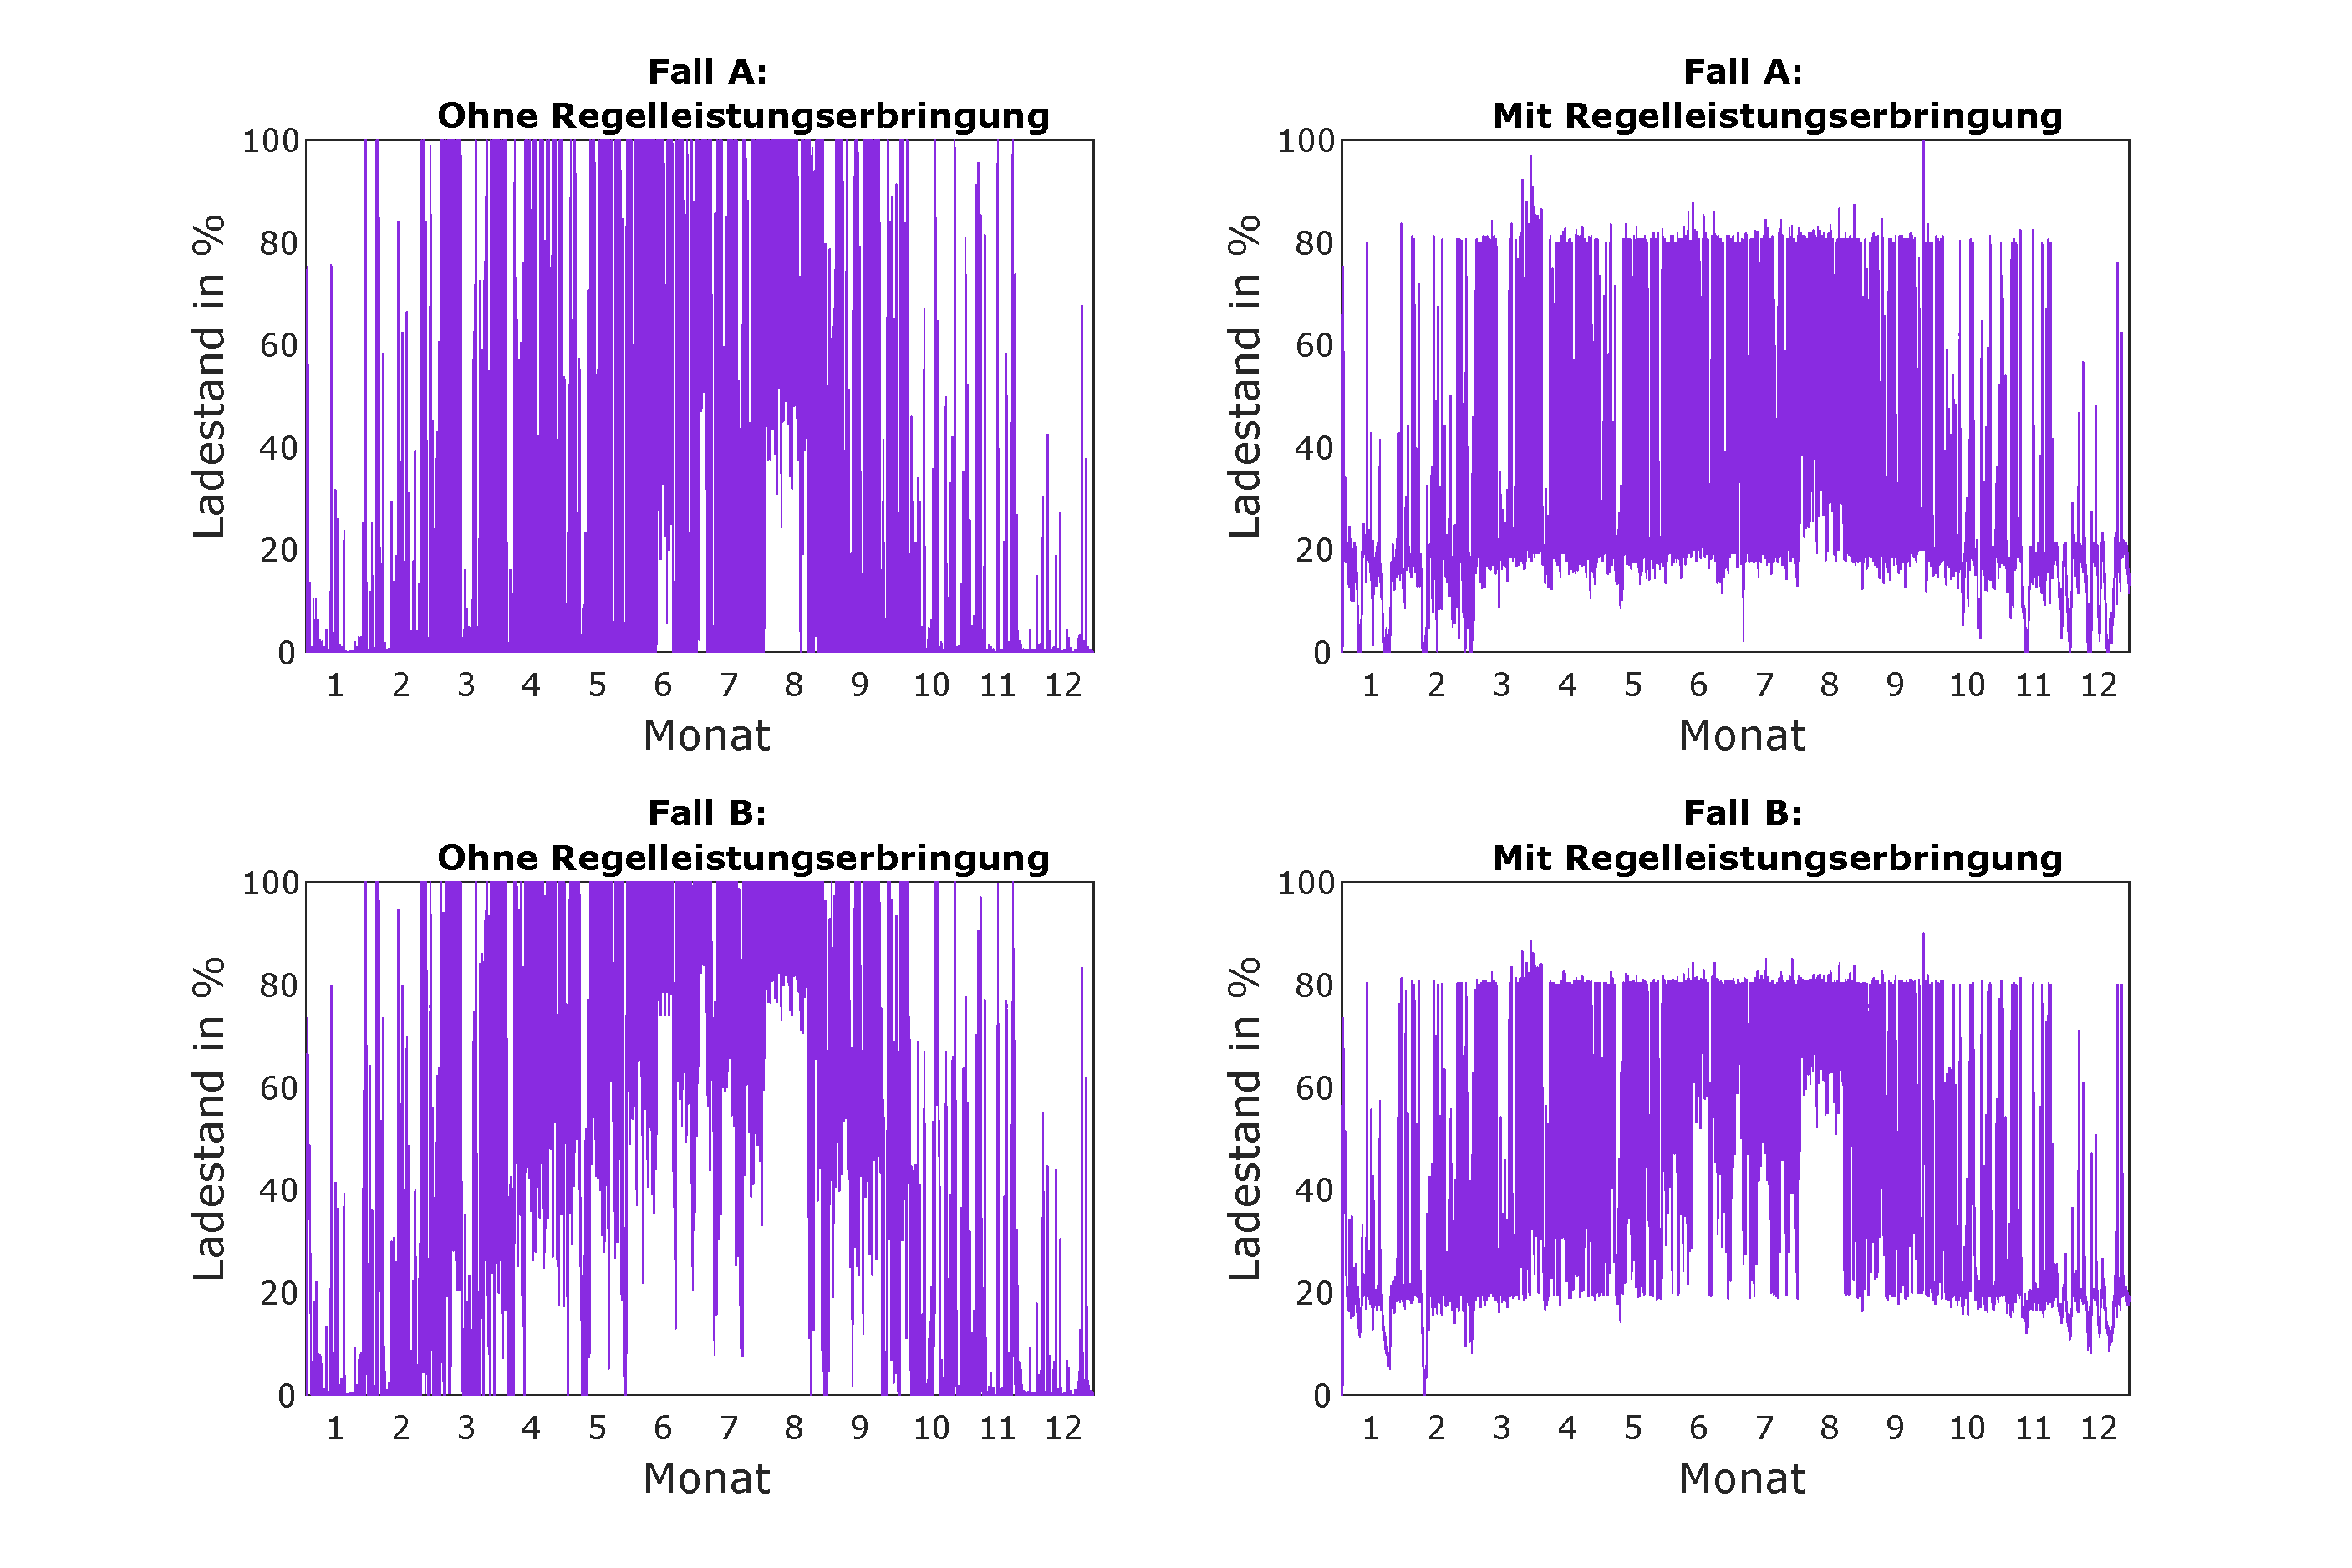
\includegraphics[width=\textwidth]{Bilder/Battery_SOC_extreme.pdf}
		\caption{Ladestandsverlauf der Fälle A und B ohne und mit Erbringung von Regelleistung. Darstellung mit durchgehend aktivierten Ladestandsgrenzen. \texttt{Eigene Darstellung}}
		\label{fig:soc}
	\end{center}
\end{figure}

\noindent In Abbildung \ref{fig:soc} sind die Ladestandsverläufe der Fälle A und B dargestellt. Damit eine optische Bewertung des Verlaufes ermöglicht werden kann, wurden für die Darstellung die Ladestandsgrenzen permanent aktiviert. Hierdurch kommt es nur durch die Erbringung von Regelleistung zu Ausschlägen ober bzw. unterhalb der Ladestandsgrenzen. Ein verschwimmen mit regelleistungsinaktiven Tagen wird hierdurch verhindert.\medskip\\
Vergleicht man die Verläufe der Fälle A und B ohne Erbringung von Regelleistung, lässt sich leicht erkennen, dass im Fall B, vor allem in den Sommermonaten, deutlich höhere Ladestandswerte auftreten. Aufgrund der höheren Photovoltaikleistung, der höheren Kapazität der Batterie und dem geringeren Hausverbrauch war dies zu erwarten.\medskip\\
Die Einschränkung des Ladestandes bei der Erbringung von Regelleistung lässt sich in beiden Fällen gut ablesen. Ausschläge ober- bzw. unterhalb der Ladestandsgrenzen gehen auf die Erbringung von Regelleistung zurück. Es zeigt sich, dass sich Ausschläge im Fall A deutlich stärker darstellen.\medskip\\
Im Fall A zeigt sich im September ein starker Ausschlag, wodurch ein Ladestand von \SI{100}{\percent} erreicht wird. An diesem Punkt kann die Batterie keine weitere Regelleistung erbringen, wodurch es zu der kleinen Abweichung in der Approximation kommt. Auch im unteren Ladestandsbereich wird häufig ein Ladestand von \SI{0}{\percent} erreicht.\medskip\\
Fall B zeigt nur geringe Ausschläge im oberen und mäßige Ausschläge im unteren Ladestandbereich. Nur im Februar wird einmalig ein Ladestand von \SI{0}{\percent} erreicht. Es kommt also nicht durch die physischen Grenzen der Batterie zu einer Abweichung von der theoretischen idealen Regelenergie, sondern durch Imperfektionen der Approximation.\medskip\\
Insgesamt zeigen sich drei Schwächen der Simulation:

\begin{enumerate}
\itemsep-0.5em
	\item Die Simulation berücksichtigt nicht, dass Primärregelleistung nur für \SI{15}{\minute} am Stück erbracht werden muss
	\item Es gibt keine Differentation zwischen der Belastung großer und kleiner Batterien, da von einem homogenen virtuellen Kratwerk ausgegangen wird
	\item Ein Lademanagement ist nicht Teil der Simulation
\end{enumerate}

\newpage
